\subsection{Shapes}

\subsubsection{Polygons}
A polygon is a shape with a finite number of straight sides and angles.\\
\begin{tabular}{rl}
    3 sides: & triangle\\
    4 sides: & quadrilateral\\
    5 sides: & pentagon\\
    6 sides: & hexagon\\
    7 sides: & heptagon\\
    8 sides: & octagon\\
    9 sides: & nonagon\\
    10 sides: & decagon
\end{tabular}\\
The sum of all interior angles of a polygon is expressed with the formula
$$\sum\theta_i=(n-2)180^\circ$$
This means that any triangle will have three angles that add to $180^\circ$ and any quadrilateral will have 4 angles that sum to $360^\circ$.\\
The area of a shape is defined to be the space enclosed by that shape.\\
The perimeter of a shape is defined to be the sum of all side lengths of that shape.

\subsubsection{Quadrilaterals}
Types of quadrilaterals:
\begin{itemize}
    \item A parallelogram is a quadrilateral with 2 pairs of parallel sides.
    $$A=bh$$
    for where $b$ is the base and $h$ is the hight. This is because a parallelogram can be constructed of two triangles with those same dimensions.
    \item A trapezoid is a quadrilateral with exactly 1 pair of parallel sides.
    $$A=\frac{h}{2}(a+b)$$
    for where $a$ and $b$ are the lengths of the two parallel sides and $h$ is the height, or distance between those parallel sides.
    \item A kite is a quadrilateral with 2 pairs of congruent (identical length) sides where the congruent sides are next to adjacent (next to another).
    $$A=\frac{1}{2}ab$$
    for where $a$ and $b$ are the lengths between opposite vertices of the kite.
    \item A rectangle is a quadrilateral with 4 right angles.
    $$A=lw$$
    \item A rhombus is a quadrilateral with 4 sides of equal length.
    $$A=bh$$
    \item A square is a quadrilateral with 4 equal sides and 4 right angles.
    $$A=l^2$$
\end{itemize}

\subsubsection{Triangles}
Types of triangles:
\begin{itemize}
    \item An acute triangle has 3 angles that each measure less than $90^\circ$
    \item A right triangle has 1 angle that measures exactly $90^\circ$
    \item An obtuse triangle has 1 angle that measures more than $90^\circ$
    \item An equilateral triangle has 3 equal side lengths.\\
    By definition, an equilateral triangle must also have all three angles be $60^\circ$.
    \item An isosceles triangle has 2 equal sides.
    \item A scalene triangle has no equal sides.
\end{itemize}
The area of any triangle can be computed using the base, $b$, and it's height (or altitude), $h$.
$$A=\frac{1}{2}bh$$
For any right angle triangle, the side lengths can be related using Pythagorean's Theorem:
$$a^2+b^2=c^2$$
for where $a$ and $b$ are two side lengths that form right angles with another and $c$ is the length of hypotenuse (the longest side).\\
A Pythagorean triple is a set of numbers that satisfies Pythagorean's theorem that are all integer values.

\subsubsection{Circles}
Every circle has a center (or origin) where the distance from the center of the circle to any part of the edge will always be the same.\\
This distance is called the radius, $r$.\\
The diameter of a circle is the length of a line running through the center that touches two points on the edge of the circle.\\
The diameter is twice the length of the radius. $d=2r$\\
The circumference of a circle is the same as its perimeter.
$$C=2\pi r$$
The area of a circle is defined as:
$$A=\pi r^2$$
A tangent line is a line that touches the edge of the circle at exactly 1 point. A tangent line will always be perpendicular to the radius.\\
A chord is a line that joins two points on a circle. Unlike the diameter, it does not need to pass through the center.\\
Arc length is some distance travelled along the outside of the circle. It can be computed as:
$$s=r\theta$$
for where $\theta$ is measured in radians.\\
A sector of a circle is a fraction of a circle, like a slice of pizza. Its area is computed as
$$A=\frac{1}{2}r^2\theta$$
\centerline{
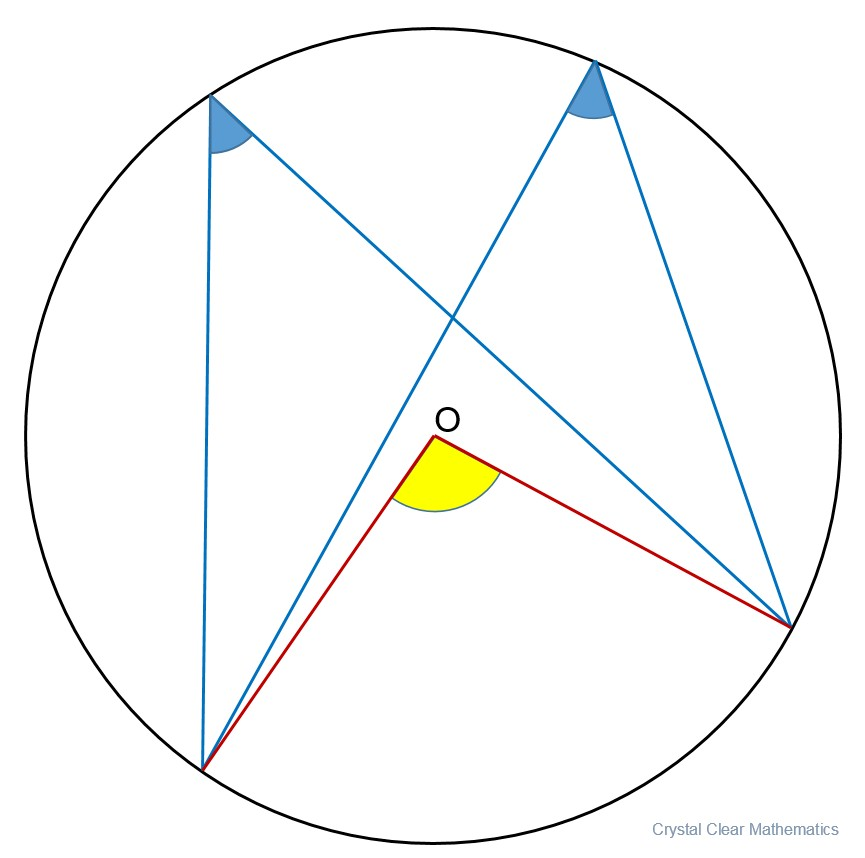
\includegraphics[scale=0.17]{Images/FundamentalsPictures/CircleGeometry.jpg}}\\
In circle geometry, the inscribed angles are shown in blue and the central angle is shown in yellow.\\
Inscribed angles subtended by the same arc are equal.\\
The central angle is twice as large as the inscribed angle.

\subsubsection{Transformations}
\begin{itemize}
    \item Symmetry:\\
    A line of symmetry is an imaginary line that divides a shape into two identical parts. Shapes are symmetrical if they have at least one line of symmetry through them.
    \item Translations:\\
    Translations are the movement of a figure from one place to another; they don't change their size, arrangement, or direction.
    \item Rotations:\\
    Rotations are when objects turn in a circular motion around a fixed pivot point. The figure remains the same, as does each point's distance from the point of rotation
    \item Reflections:\\
    A reflection is a transformation that acts like a mirror: it swaps all pairs of points that are on exactly opposite sides of the line of reflection.
    \item Dilations:\\
    A dilation is a type of transformation that changes the size of the figure. The scale factor measures how much larger or smaller the image is. The angles remain the same.
    \item Congruence:\\
    Shapes are congruent with another if they are the same size and shape (same angles). Transformations can be applied to similar shapes to see if they can become congruent.
    \item Similarity:\\
    Two shapes are similar if a series of transformations can be applied to one in order to achieve the other. Similar shapes will always have matching angles.
\end{itemize}

\subsubsection{3D Shapes}
The volume of a shape is the 3D space that the object takes up.\\
The surface area is the sum of the areas of the shape's exterior.
Common 3D shapes:
\begin{itemize}
    \item A cube has all equal side lengths and equal square faces.
    $$V=l^3$$
    $$SA=6l^2$$
    \item A prism has two identical faces on each end, connected by a straight body.
    $$V=A_{base}h$$
    \item A pyramid has the vertices at the base come together to form a point above the base. Note that a cone is a special type of pyramid with a circular base.
    $$V=\frac{1}{3}A_{base}$$
    \item A sphere is entirely circular.
    $$V=\frac{4}{3}\pi r^2$$
    $$SA=4\pi r^2$$
\end{itemize}